% Source-faithful schematic draft: 2004 Chongqing Science Q15, PDF p.1 (printed p.160).
% Source ID: src-f4f7a5339a68a3cbcf5ef54e4d3736a907b6de9c04c1ef9f3f8b8f7b718d56c4
% Source SHA-256: ef3530a818ad893a36345110d6aa9588de3b793de24c4d6f80333cffa317e429
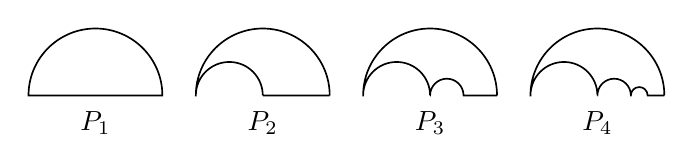
\begin{tikzpicture}[line width=0.6pt, scale=0.85, every node/.style={inner sep=1.5pt}, baseline=(current bounding box.center)]
  % P1: Complete semicircle of radius 1
  \begin{scope}[shift={(0, 0)}]
    \draw (0, 0) -- (2, 0) arc[start angle=0, end angle=180, radius=1] -- cycle;
    \node[below=4pt] at (1, 0) {$P_1$};
  \end{scope}

  % P2: Semicircle with a smaller semicircle of radius 1/2 cut from left
  \begin{scope}[shift={(2.5, 0)}]
    \draw (1, 0) arc[start angle=0, end angle=180, radius=0.5] -- (0, 0) arc[start angle=180, end angle=0, radius=1] -- (2, 0) -- (1, 0);
    \node[below=4pt] at (1, 0) {$P_2$};
  \end{scope}

  % P3: Semicircle with second cut of radius 1/4
  \begin{scope}[shift={(5.0, 0)}]
    \draw (1, 0) arc[start angle=0, end angle=180, radius=0.5] -- (0, 0) arc[start angle=180, end angle=0, radius=1] -- (2, 0) -- (1.5, 0) arc[start angle=0, end angle=180, radius=0.25] -- (1, 0);
    \node[below=4pt] at (1, 0) {$P_3$};
  \end{scope}

  % P4: Semicircle with third cut of radius 1/8
  \begin{scope}[shift={(7.5, 0)}]
    \draw (1, 0) arc[start angle=0, end angle=180, radius=0.5] -- (0, 0) arc[start angle=180, end angle=0, radius=1] -- (2, 0) -- (1.75, 0) arc[start angle=0, end angle=180, radius=0.125] -- (1.5, 0) arc[start angle=0, end angle=180, radius=0.25] -- (1, 0);
    \node[below=4pt] at (1, 0) {$P_4$};
  \end{scope}
\end{tikzpicture}
